\chapter{Etat de l'art}
\label{part:etat_art}

Les relations qui peuvent exister entre la partie invisible de la performance et la performance elle-même ont suscité beaucoup d'intérêt. Voici un état de la littérature existante proposant des résultats intéressants et complémentaires à l'expérimentation qui va suivre.\\

La concentration sanguine de lactate est un des paramètres physiologiques qui a bénéficié du plus grand nombre d'articles de recherche, car la lactatémie est un des facteurs qui influence le plus la performance au 400 mètres.\\

   \section{Normes de la concentration de lactate}
       
       Selon l'étude de O. BANG \cite{bang36}, la concentration sanguine de lactate au repos est en moyenne de 1.94 mmol/l (fig. \ref{fig:lactate_repos}).\\
       
       \begin{figure}[H]
                \centering
                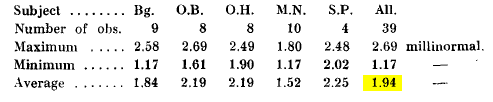
\includegraphics[scale=1]{images/lactate_repos.PNG}
                \caption{\label{fig:lactate_repos}Concentration sanguine de lactate au repos.}
        \end{figure}
        
       Pour F. PERONNET \cite{peronnet13}, les exercices courts et intenses comme le 400 mètres reflètent l'accumulation de grandes quantités de lactate qui peuvent avoisiner 30 mmol/l.
        
    \section{Effet de l'intensification de l'effort sur la lactatémie}
    
       Différentes études ont mis en évidence le fait que la lactatémie augmente progressivement au fur et à mesure que l'exercice s'intensifie.\\
       
       T. E.GRAHAM \cite{graham84} et A. P.CHASSAIN \cite{chassain86} ont tous deux étudiés l'évolution de la concentration du lactate sanguin lors de l'augmentation du pourcentage de V02max, c'est à dire à 60, 70 et 90\% de l'absorption maximale d'oxygène du sujet par exemple (fig. \ref{fig:lactate_vo2max}).\\
       
       \begin{figure}[H]
                \centering
                \fbox{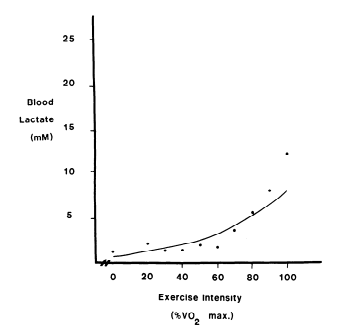
\includegraphics[scale=0.7]{images/lacta_vo2max.PNG}}
                \hfill
                \fbox{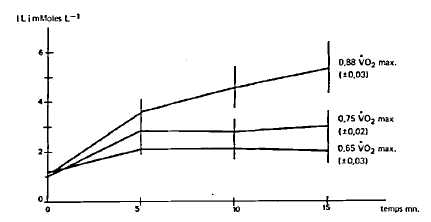
\includegraphics[scale=0.8]{images/lactate_vo2max3.PNG}}
                \caption{\label{fig:lactate_vo2max}
                La réponse du lactate sanguin à l'augmentation du pourcentage du VO2max. (Résultats de GRAHAM à gauche et CHASSAIN à droite).}
        \end{figure}
        
        T. E.GRAHAM et  A. P.CHASSAIN ont démontré que plus l'intensité de l'exercice augmente, c'est à dire que plus le sujet se rapproche de son VO2Max, plus sa concentration sanguine de lactate augmente. La lactatémie augmente significativement à partir de 60\% de la VO2Max.\\
      
       M. L. GOODWIN \cite{goodwin07} a quant à lui étudié l'évolution de la lactatémie lors de l'augmentation de la force générée c'est à dire du seuil de travail (calculé en watt) (fig. \ref{fig:lactate_work_rate}). L'exercice mis en place pour cette étude était de produire un effort de 4 minutes et d'augmenter l'intensité de 30W chaque minute. Les échantillons de sang étaient prélevés durant les 30 dernières secondes de chaque seuil de travail via un cathéter placé dans l'avant bras du sujet.\\
       
       \begin{figure}[H]
                \centering
                \fbox{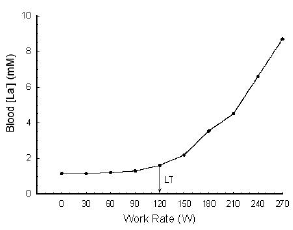
\includegraphics[scale=1]{images/lactate_work_rate}}
                \caption{\label{fig:lactate_work_rate}
                La réponse du lactate sanguin à l'augmentation du seuil de travail.}
        \end{figure}
        
        
        Enfin, dans leur étude, J. R. LACOUR et coll.\cite{lacour90} ont mesuré la lactatémie de 17 athlètes de haut niveau après des courses de 400 mètres. Les résultats qu'ils ont obtenus montrent que l'augmentation de la vitesse provoque également une hausse de la lactatémie (fig. \ref{fig:lactate_vitesse}).\\
    
          \begin{figure}[H]
                \centering
                \fbox{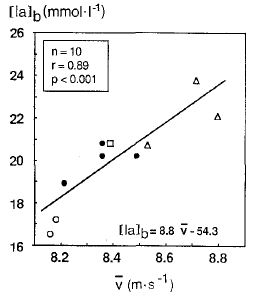
\includegraphics[scale=1]{images/lactate_vitesse}}
                \caption{\label{fig:lactate_vitesse}
                La réponse du lactate sanguin à l'augmentation de la vitesse.}
        \end{figure}
        
       
        Ainsi, quelque que soit la méthode utilisée, les recherches indiquent que la lactatémie augmente graduellement au début de l'exercice puis significativement lorsque l'effort devient plus intense. Ceci est expliqué par le fait que lors de l'exercice intense, ce sont les processus métaboliques anaérobies (sans oxygène) qui tiennent la place la plus importante. Le déficit en oxygène augmente donc progressivement, ce qui détermine une augmentation progressive de la concentration sanguine de lactate.\\

        
    \section {Lactatémie maximale après effort}
    
        Les résultats publiés par M. L. GOODWIN \cite{goodwin07} montrent que la concentration de lactate sanguin est la plus élevée dans les 3 à 8 minutes suivant la fin de l'exercice (fig. \ref{fig:lactate_recup}).
            
            \begin{figure}[H]
                \centering
                \fbox{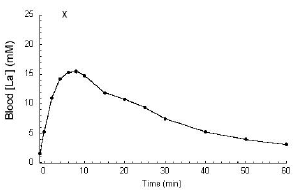
\includegraphics[scale=1]{images/lactate_recup}}
                \caption{\label{fig:lactate_recup} Évolution de la lactatémie après la fin de l'effort.}
             \end{figure}
            
        
        La plupart des études portant sur la lactatémie de fin de course ont été réalisées sur les disciplines de 400, 800 et 1500 mètres, car comme le montrent J.R LACOUR et coll.             \cite{lacour90}, ce sont elles qui mettent en jeu le métabolisme anaérobie lactique de façon la plus importante.\\
    
    
    \section{Lactatémie et performance}
        
        Dans la même étude, J.R LACOUR et coll. \cite{lacour90} se sont également attachés à déterminer s'il existait une relation entre la lactatémie et la performance, c'est à dire le temps réalisé au 400 mètres. Pour ce faire, ils ont mesuré la concentration sanguine de lactate à l'issue de courses de 400 mètres réalisées par des athlètes de niveau national et international lors de compétitions majeures comme les championnats de France, d'Europe et du Monde. Les échantillons ont été prélevés entre 5 et 10 minutes après la fin de l'effort et les résultats obtenus ont ensuite été mis en relation avec les meilleures performance de la saison de chaque athlète pour déterminer si une dépendance existait.\\           
        
        Les résultats montrent une corrélation systématique entre les performances réalisées et la concentration sanguine de lactate (r=0.89, P<0.01). Plus le temps réalisé par l'athlète se rapproche de sa meilleure performance de la saison, plus sa lactatémie augmente (fig. \ref{fig:lactate_velocite}). 
        
         \begin{figure}[H]
            \centering
            \fbox{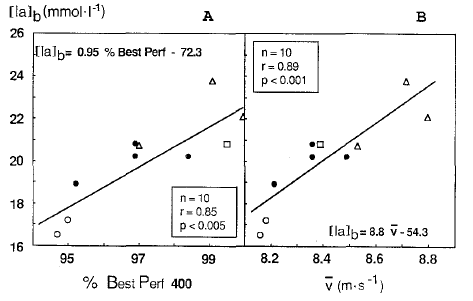
\includegraphics[scale=1]{images/lactate_velocite}}
            \caption{\label{fig:lactate_velocite} Évolution de la lactatémie post-effort.}
        \end{figure}
        
        Selon eux, les athlètes qui réussissent le mieux dans les exercices courts (de 10 secondes à 5 minutes) sont ceux qui produisent le plus de lactate et par conséquent, fournissent à leurs muscles le plus d’énergie par unité de temps. De la même façon, G.CAZORAL et coll. \cite{cazorla01} ont mis en évidence le fait que « ce n’est pas un hasard non plus si le guépard qui peut courir à 100 km/h est un très gros producteur de lactate ».  \\        
    

    \section {Fréquence cardiaque et SPO2}

        H. TABATABAEI \cite{tabatabaei00} s'est attaché à rechercher s'il existait une relation entre la SPO2 et la fréquence cardiaque.\\
        
        Les sujets de cette étude étaient une équipe national de canoe, de Taekwando, de lutte de des athlètes spécialistes des distances moyennes. Le test consistait à courir sur un tapis de course à la vitesse de 8 km/h au début, puis la vitesse augmentait de 1 km/h chaque minute jusqu'à épuisement. \\
        
        Les résultats indiquent que les deux variables sont bien corrélées, car plus la fréquence cardiaque est élevée, plus la saturation pulsée en oxygène est faible (fig. \ref{fig:spo2_fc}).\\
     
         \begin{figure}[H]
            \centering
            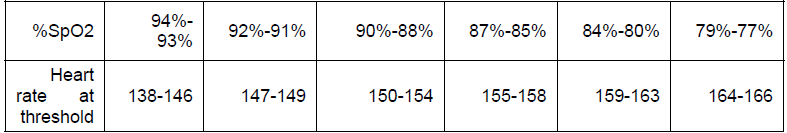
\includegraphics[scale=0.8]{images/spo2_fc.PNG}
            \caption{\label{fig:spo2_fc} Relation entre la fréquence cardiaque et la SpO2 pendant l'effort.}
        \end{figure}
        
        D. LAIN et coll. \cite{lain13} ont mené une étude similaire, mais à vélo, et ont observé qu'à partir d'une fréquence cardiaque environ égale à 170 bpm, la saturation pulsée en oxygène chute brutalement (fig. \ref{fig:spo2_fc2}.)
        
         \begin{figure}[H]
            \centering
            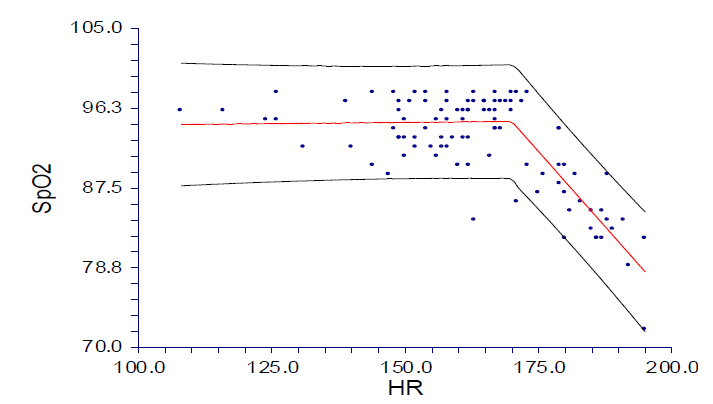
\includegraphics[scale=0.6]{images/spo2_fc2.PNG}
            \caption{\label{fig:spo2_fc2} Relation entre la fréquence cardiaque et la SpO2 pendant l'effort.}
        \end{figure} 
        

    \section{Étude de la glycémie après effort}
        
        Les effets d'un sprint court sur les taux de production et d'utilisation du glucose dans le corps a suscité plusieurs recherches.\\

        A.J. FAHEY et coll. \cite{fahey12} ont montré qu'un exercice maximal de seulement 10 secondes est capable de provoquer une augmentation des concentrations de glucose sanguin chez les individus en bonne santé (fig.\ref{fig:glycemie_posteffort}).\\
        
        \begin{figure}[H]
            \centering
            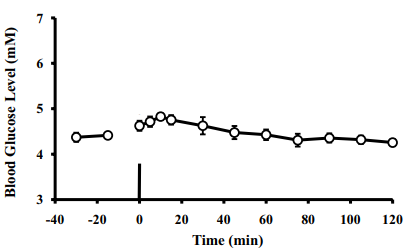
\includegraphics[scale=0.9]{images/glycemie_posteffort.PNG}
            \caption{\label{fig:glycemie_posteffort} Évolution de la glycémie en réponse à un sprint de 10 secondes (représenté par la barre verticale).}
        \end{figure} 

        Les résultats de l'étude effectuée par T.D. JUSTICE et coll. \cite{justice15} confirment ces résultats et indiquent que la glycémie augmente aussi après un sprint maximal de 30 secondes. Dans cette étude ils démontrent également qu'un exercice antérieur d'intensité modérée atténue l'effet d'augmentation de la glycémie d'un effort intense.
        
        \begin{figure}[H]
            \centering
            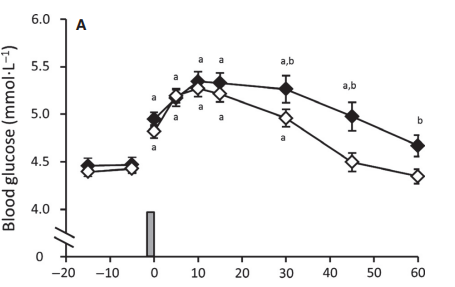
\includegraphics[scale=0.9]{images/glycemie_posteffort2.PNG}
            \caption{\label{fig:glycemie_posteffort2} Réponse de la glycémie à un sprint de 30 secondes (représenté par la barre verticale) réalisé après 60 minutes d'exercice d'intensité  modérée (losanges blancs) ou sans cet exercice (losanges noirs).}
        \end{figure} 
        
         Les niveaux de glycémie augmentent de manière significative et similaire dans les deux essais en réponse au sprint, atteignant un pic à 10 minutes de récupération. La glycémie a ensuite diminué plus rapidement lorsque que les sujets avaient effectué un exercice antérieur d'intensité modérée.


%%% Local Variables: 
%%% mode: latex
%%% TeX-master: "rapport"
%%% End: 
